\chapter{RNA Motifs}
\label{motifs} 
\bibliographystyle{nar} As mentioned  in pages 24 and 25  of Chapter 2
the most  common perspectives for RNA motif  recognition and discovery
are the atom and bond based ones, the rigid-body-based perspective has
been rather  unexplored.  The  two main questions  that we  address in
this context are:

\begin{enumerate}
\item{Can  the geometric rigid-block  description of  base-pairing and
  base-stacking solve the problem of defining RNA structural motifs?}
\item{Can other  quantities derived from the 3DNA  software package be
  used to make an automated search for known motifs, for example, the
  GNRA tetraloop motif, and perhaps find unknown motifs?}
\end{enumerate}

We start with the  second question and have chosen as workhorse
the  well  known  GNRA  tetraloop  motif.  We  also  used  other
quantities  (e.g.  endocyclic  and  exocyclic base-overlaps)  obtained
with the 3DNA \cite{lu2003, lu2008b} package to  complement the
automated search for GNRA tetraloop motifs.

\section{The GNRA Tetraloop}
The GNRA motif  was initially found to be  an important constituent of
the small subunit  of the ribosome using the  technique of comparative
sequence analysis \cite{woese1990}, that is, it was seen that the GNRA
sequence was frequently repeated  among various organisms in tetraloop
regions of RNA, and so were  the CUUG and UNCG tetralops, which amount
to  more than  70\% of  all  tetraloops found  in the  16S subunit  of
ribosomal RNA \cite{woese1990, depaul2010}.   The most abundant of all
the tetraloops in  the ribosome is the GNRA  motif, and its structural
stability was  initially characterized using NMR  spectroscopy by Heus
and  Pardi \cite{heus1991}  who determined  that the  loops  contain a
non-canonical  sheared G$\cdot$A  base-pair flanking  the  sequence, a
hydrogen bond between  a guanine base and a  phosphate, extensive base
stacking, and a  hydrogen bond between the hydroxyl  group of a ribose
and  a base  \cite{heus1991},  such  features can  be  seen in  Figure
\ref{fig:gnrablocks}.

\begin{figure}
\centering
%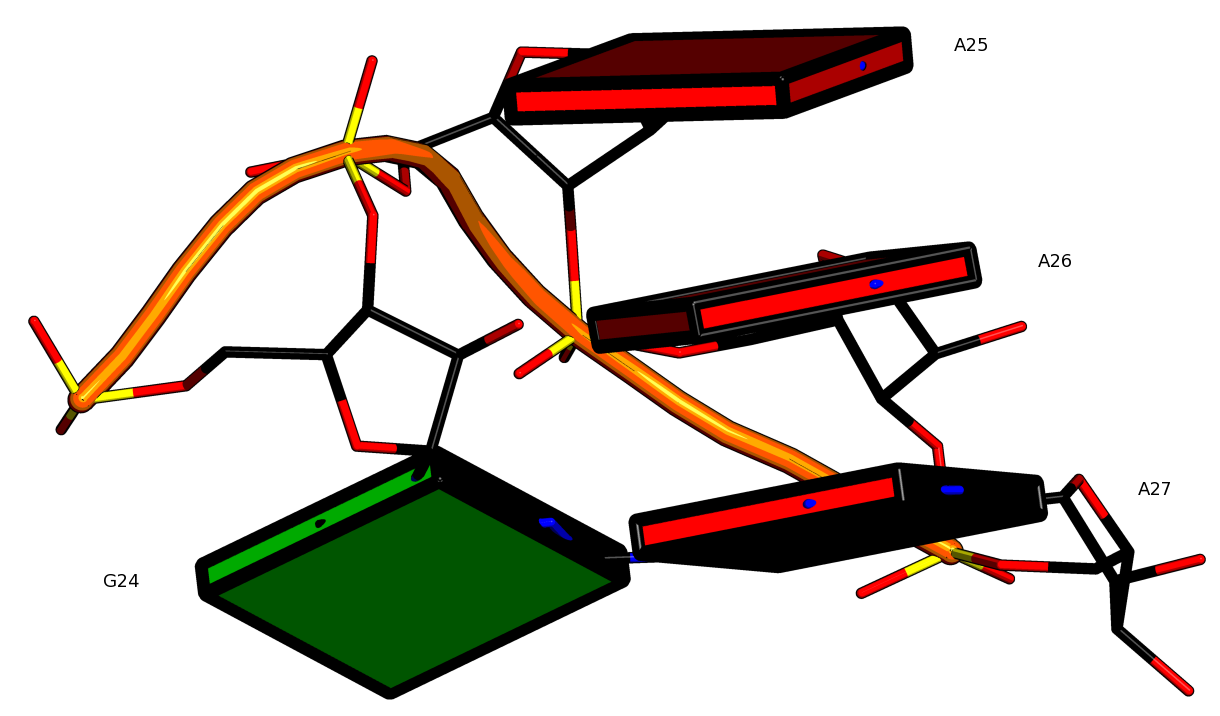
\includegraphics[angle=0]{Chapter5/gnra24.png}
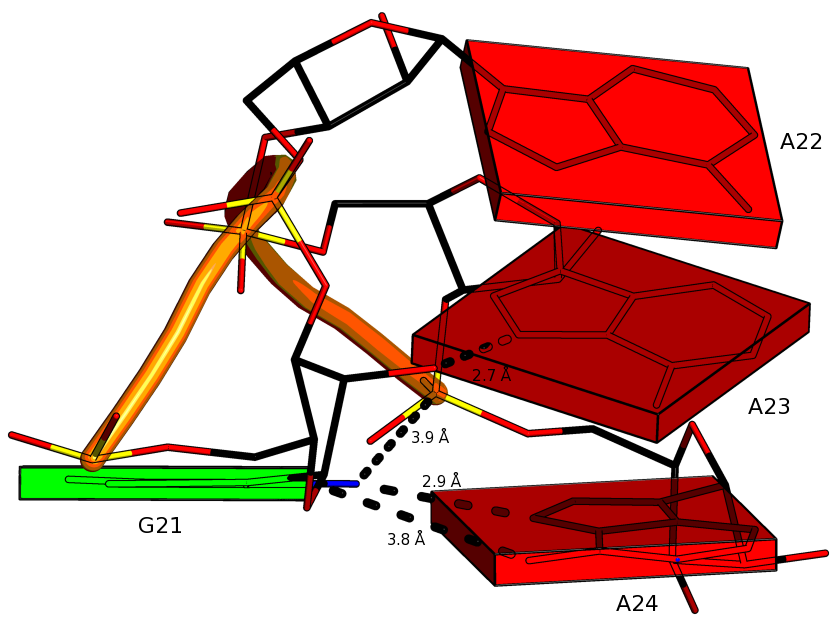
\includegraphics[angle=0, scale=0.38]{Chapter5/gnra21L2.png}
\caption{The   GNRA  tetraloop  motif   in  the   hammerhead  ribozyme
  PDBIB:1hmh  \cite{pley1994}  although not  a  newly recognized  GNRA
  tetraloop,   it's  positively   recognized   using  our   rigid-body
  parameters RNA motif search  program ``getMotif''. The structure was
  selected from a non-redundant list of RNA structures provided by the
  RNA  ontology consortium (ROC).   The hydrogen  bonding interactions
  described  by  Heus and  Pardi  \cite{heus1991}  as  results of  NMR
  experiments are shown in black dashed lines.}
\label{fig:gnrablocks}
\end{figure}

The description of  the GNRA tetraloop motif is a  typical case of the
problem  of RNA  motif  definition,  for example,  in  the context  of
sequence  alone  a  GNRA  motif  would  be one  which  follows,  in  a
consecutive manner, the GNRA pattern, whereas it has been noticed that
there can be GNRA structures which are not consecutive in sequence but
have  the same  geometric  arrangement of  bases in  three-dimensional
space  as  the  sequentially   linked  GNRA  motif.   There  are  also
structures  which posses the  same geometric  arrangement as  the GNRA
tetraloop, and are also arranged sequentially (i.e.  are connected
covalentently  through  their sugar-phosphate  backbone),  but do  not
follow the  same sequence pattern,  for example the UCAA,  UCAC, CAGA,
and  CAAC tetraloops\cite{lemieux2006}.   These other  sequences which
are  geometrically  equivalent to  the  GNRA  tetraloop  motif form  a
non-canonical base-pair which is isosteric to the G$\cdot$A base-pair,
that is, the U$\cdot$A, U$\cdot$C, C$\cdot$A, and C$\cdot$C base-pairs
closing the  tetraloops are isosteric  to the G$\cdot$A  base-pair, as
was found by Lemieux and Major \cite{lemieux2006}.

Some   studies   have  used   molecular   dynamics   to  explore   the
conformational space of  the GNRA tetraloop. These studies  find a set
of conformational states for the  GNRA tetraloop motif which are later
related to existing X-Ray and  NMR structures available at the protein
data bank \cite{depaul2010, sorin2002}. Other MD studies have used the
well known GNRA motif conformation as starting point for simulation of
other tetraloops.   These other  tetraloops turn out  not to  retain a
GNRA-like three-dimensional  structure \cite{srinivasan1998}, but this
effect might  just be due  to the fact  that the force fields  used in
such  calculations \cite{cornell1995}  seem  not to  be  able to  make
correct predictions for  tetraloops as has been show  recently for the
GAAA tetraloop \cite{spackova2010}.

\subsection{GNRA Motif Search Program}
We have  devised a simple algorithm to search for GNRA  motifs based on
their base  step parameters.  The  algorithm is illustrated  in Figure
\ref{fig:getMotif}.

\begin{figure}
\centering
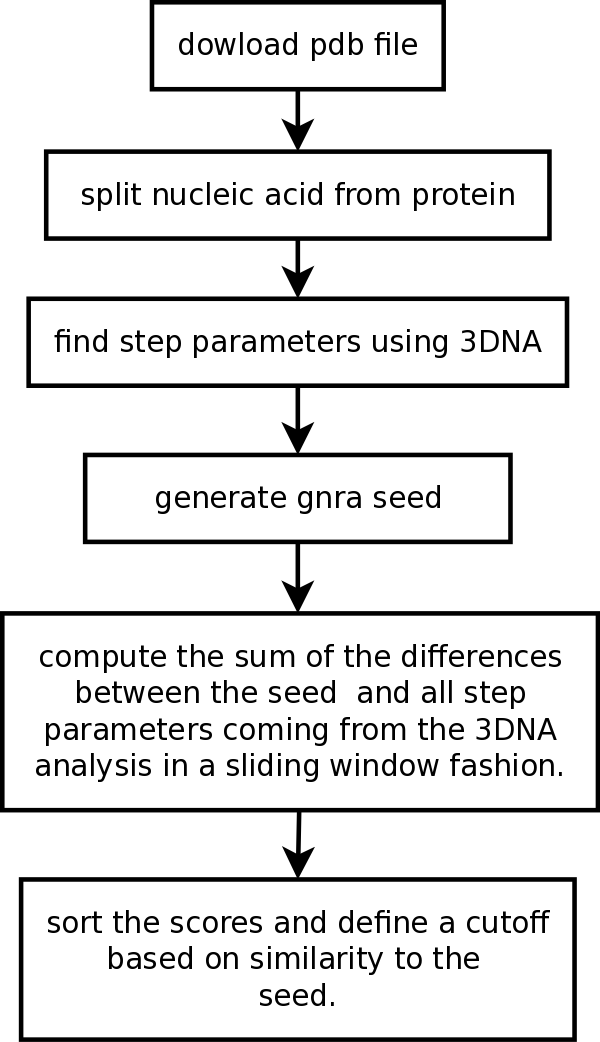
\includegraphics[angle=0, scale=0.4]{Chapter5/getMotif.png}
\caption{Simple algorithm  for GNRA motif  finding based on  base step
  parameters.}
\label{fig:getMotif}
\end{figure}
  
The algorithm  allows for any  motif seed to  be used, but for  now we
only use the step parameters of the GNRA motif as the seed for our
algorithm.   We are  currently  constructing a  database of  base-step
parameters for  known motifs, so  that our simple  program ``getMotif''
can be expanded  to include various known motifs  the user wishes
to localize in a given RNA structure.

The  algorithm has  been programed  as a  simple, yet  very  fast bash
script which interfaces with  three components, one written in python,
another is the 3DNA package, and another is written in the statistical
analysis  software R.   For  example,  for the  large  subunit of  the
ribosome, PDB-ID:1jj2, the program  takes 22.1 seconds to download and
analyze the whole  structure in an Intel Core Duo  of 2.13GHz with 8Gb
of RAM.

The  program, which  we have  called ``getMotif'',  allows the  user to
query any PDB\_ID. That is, the user only needs to input in the command
line of a UNIX/LINUX terminal the command, ``getMotif'' followed by the
PDB\_ID of the RNA molecule of interest. As a result the user obtains a
list composed of residue numbers  corresponding to the location of the
start of the motif in the  structure, and a score which stands for how
close or far  a four nucleotide sequential structure  is from the GNRA
motif seed.   The advantage  of our program  over other  windows based
motif  recognition softwares,  besides from  providing a  new analysis
based on rigid-body parameters, is that it allows for easy integration
of  automated  scripts  for   processing  large  lists  of  known  pdb
structures  without  user  intervention   for  the  analysis  of  every
structure. For  example, in the RNA ontology  consortium (ROC) meeting
of  May  2009   a  reduced  dataset  of  RNA   structures  found  at:
\url{https://docs.google.com/Doc?id=dhrmkfmn_13ftpbjcgq}    was   made
available to participants with the  purpose of allowing them to search
for RNA  motifs which  would later be  compared between  groups. Using
windows  based  softwares   like  FR3D  \cite{sarver2008}  it's  quite
difficult,  if not  impossible, for  the user  to submit  a  large job
composed  of many  pdb structures  to a  queing system,  or  a cluster
computing server, such task is made simple using getMotif.

To construct  the seed for  the GNRA motif  we extracted the  first 20
GNRA tetraloop motifs found by Lemieux and Major \cite{lemieux2006} in
the large subunit of the ribosome (PDB-ID:1ffk) as show in Figure 3 of
their results. After computing the  base step parameters with 3DNA for
each of these motifs we arrange their average values in a 3 x 6
matrix $S$ where each row corresponds to one of the three steps in the
tetraloop. These average values are show in Table \ref{tab:seed}.

\begin{table}[hb]  
\begin{center}
\begin{tabular}{|c|c|c|c|c|c|c|}
\hline
Step & Shift & Slide & Rise & Tilt & Roll & Twist \\
\hline
GN & -9.77 & -1.90 & -4.93 & 71.8 & 124.0 & -57.5 \\
NR & 2.74 & -0.11 & 3.04 & 11.5 & 6.0 & 50.6 \\
RA & 1.11 & -0.20 & 3.01 & 9.5 & 6.1 & 42.4 \\
\hline
\end{tabular}
\caption{GNRA motif  seed composed of the average  base step parameter
  values for 20 GNRA motifs found in the large subunit of the ribosome
  PDBID:1ffk \cite{lemieux2006}.}
\label{tab:seed}
\end{center}
\end{table}

We  then  compute  a  score  to determine  the  distance  between  all
sequences formed by  three sequential steps in a  given RNA structure,
and the GNRA  motif seed. The score is simply the  sum of the elements
of the difference matrix $X_{k}$,  where the difference is between the
GNRA matrix $S$ and each one of the $k-3$ sequential 3 x 6 matrices
$W_{k}$, where $k$ is the total number of steps in the RNA structure.

\begin{gather}
X_{k} = |S - W_{k}| \\
\text{score}_{k} = \sum X_{m,n} 
\end{gather}  

The scores  obtained from analysis  of the large ribosomal  subunit of
the  ribosome PDBID:1ffk  can be  seen in  the histogram  displayed in
Figure \ref{fig:gnrahist}.

\begin{figure}
\centering 
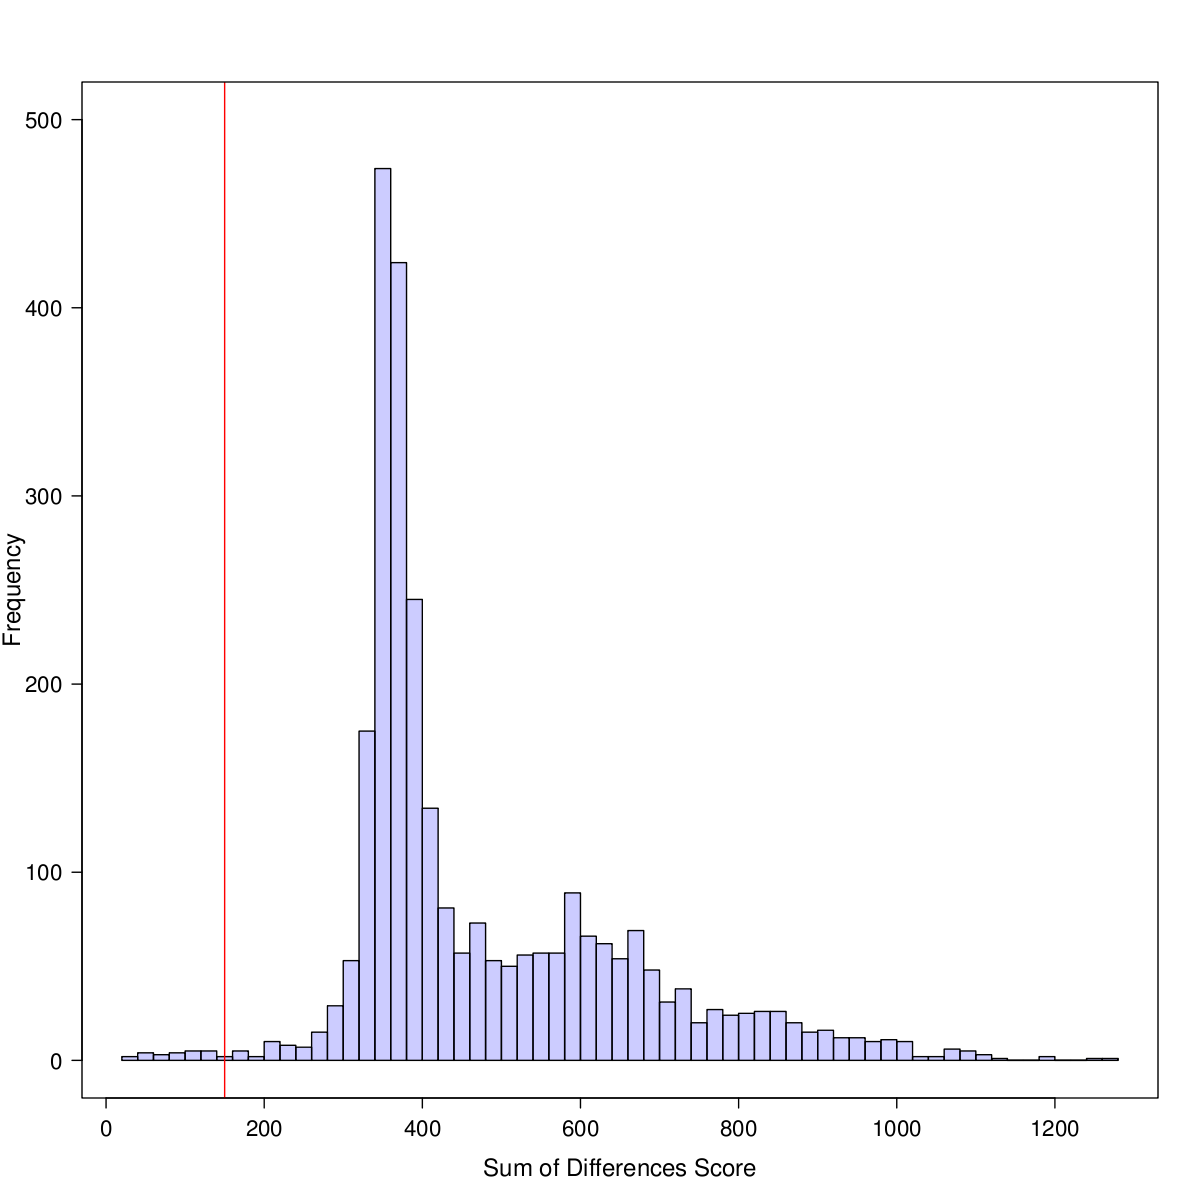
\includegraphics[angle=0, scale=0.5]{Chapter5/gnrahisto.png}
\caption{Histogram for  the sum of differences score  between the GNRA
  motif seed and  all sequential tri-steps found in  the large subunit
  of the ribosome PDBID:1ffk}
\label{fig:gnrahist}
\end{figure}

In this histogram we see that the majority of scores have a peak value
in bin 8,  which corresponds to scores between  350-400, these values
correspond to tri-step sequences located withing helical regions which
are  more or less  evenly distant  from the  GNRA tetraloops.  For our
purposes of GNRA  motif identification we want to  select those scores
which reflect a shorter distance  to our seed GNRA motif, therefore we
have used  a cutoff of  150 in our  score which is represented  by the
values below the red vertical line in Figure \ref{fig:gnrahist}.

Using our program in a list of 355 RNA structures provided by the ROC,
and the  selected cutoff  value of 150  we find \footnote{The  time it
  took to search for GNRA tetraloop motifs in the 355 structures was 7
  minutes  and 29 seconds}  that 75  out of  these 355  structures are
identified as having at least one GNRA 3D motif candidate, and a total
of 211  GNRA motif candidates.  The  list of all  identified motifs in
these 75  structures is shown in Table  \ref{tab:gnrascores}, where an
additional  check for consistency  is that  of having  zero endocyclic
overlap in the first step of the tetraloop, as can be seen in the next
to last column of the table.   We also see that 67\% of the identified
GNRA motif candidates start with  a GN step, and interestingly, almost
one third  (27\%) of the first  steps identified are UN  steps, also a
few of the identified motifs start with AN and CN steps.

To  further  analyze the  result  of  identification  of motifs  using
``getMotif'' we focused our  attention on the ribosomal structure with
PDBID:2jo1 which is included in the ROC list.  As can be seen in Table
\ref{tab:gnrascores} for the 2jo1 entry, the program recognizes twenty
GNRA tetraloop motif candidates, which  are all in fact tetraloops, 13
of them conform to the GNRA sequence, 5 start with UN, one starts with
A and  one with C.  When  we align the GNRA  motif candidate sequences
using the  reference frame  of the  first two bases  we see  that they
belong to two main groups, one with about eleven members and the other
with 7  members, the two remaining  structures fit well  the first two
steps, with  both groups I and  II, but do  not fit well on  the third
step. In Figure \ref{fig:groupsB} we show the two main groups. Group I
is colored in blue,  and we see that this one is  closer to the common
GNRA motif, and  Group II is colored in red. Group  II loops are close
to being  a common GNRA motif, but  insted they have a  larger rise in
the  last step,  nonetheless  the  first two  steps  are very  closely
related in every  case, in a sense  it looks as if there  was a subtle
switching  between  being a  triloop,  a  tetraloop,  or a  pentaloop,
governed by the rise in the last step.

\begin{figure}
\centering 
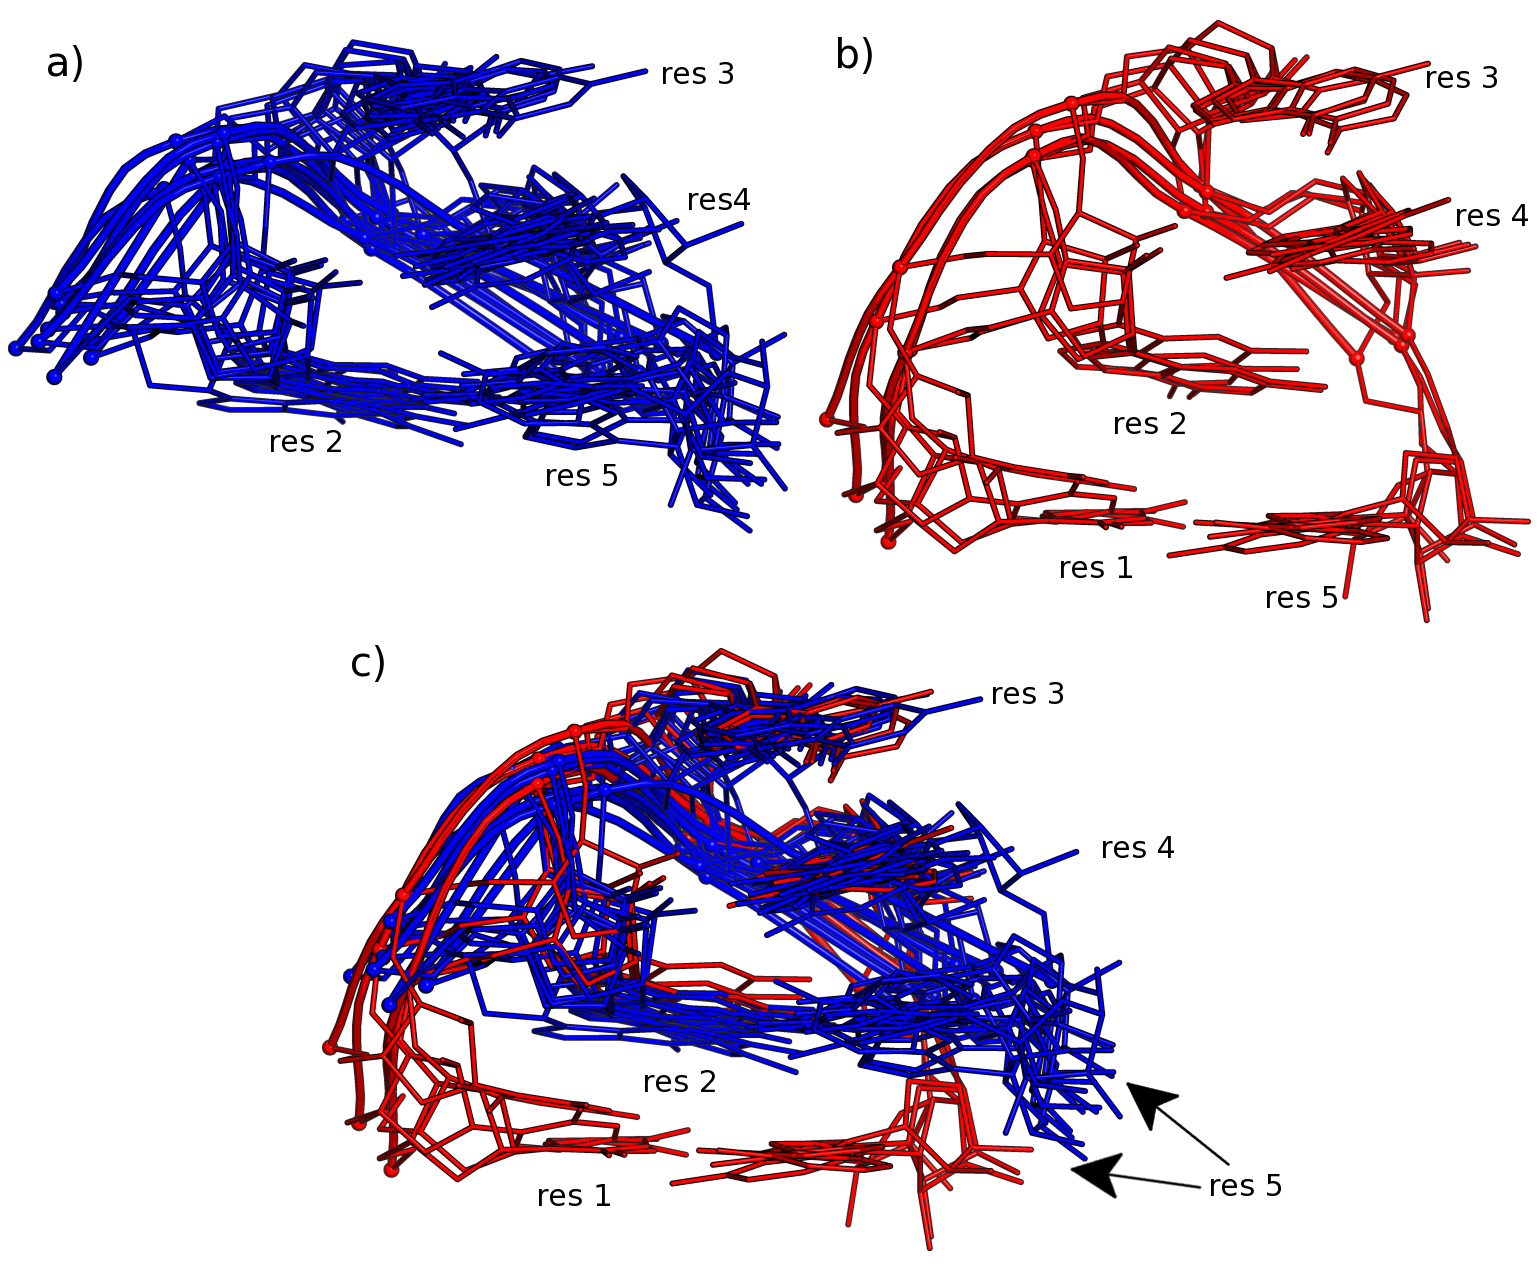
\includegraphics[angle=0, scale=0.5]{Chapter5/groupsB.png}
\caption{Scatterplot  of  base-step parameter  values  for GNRA  motif
  candidates identified in a list given by the ROC, against a backdrop
  of the range of values  for the step-parameters in the large subunit
  of the ribosome PDBID:1ffk.}
\label{fig:groupsB}
\end{figure}


Interestingly in the  GNRA candidates identified in group  II they are
part    of   a    highly   symmetrical    extended    loop   "kissing"
interaction. These can be seen in figure where they are supperimposed,
and in their orirginal orientation in the ribosome.

From the three steps which make up the GNRA tetraloop the first one is
the  one farthest away  from a  typical ARNA  type base-step,  we have
plotted the step-parameter values for this first step in a scatterplot
\ref{fig:scattergnra}, where it's clear  that this steps constitutes a
well  defined  region  in  the  space  of  rigid-body  step  parameter
configuration space for the large subunit of the ribosome.

\begin{figure}
\centering 
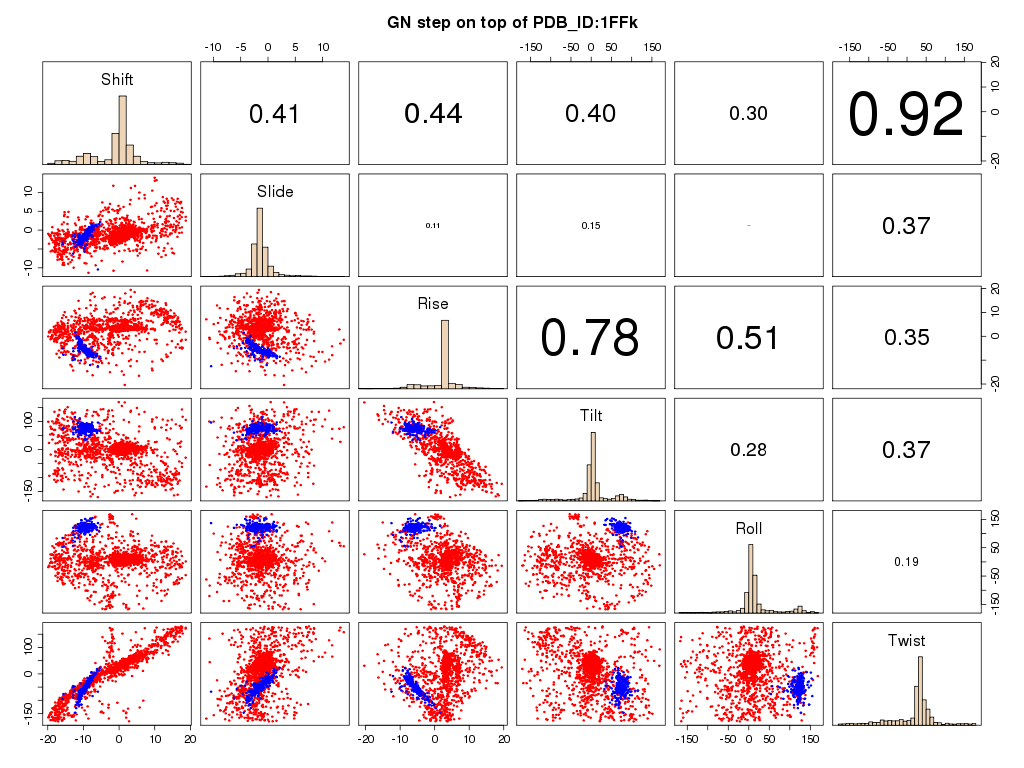
\includegraphics[angle=0, scale=0.5]{Chapter5/GNRAin1ffk.png}
\caption{Scatterplot  of  base-step parameter  values  for GNRA  motif
  candidates identified in a list given by the ROC, against a backdrop
  of the range of values  for the step-parameters in the large subunit
  of the ribosome PDBID:1ffk.}
\label{fig:scattergnra}
\end{figure}

%\section{Canonical "Noise"}
%To be able to say anything about motifs it's crucial to get rid of the
%"noise" which is given by the canonical base-pair steps.
%One would think that perhaps  the X3DNA-Parser of Dr. Yurong Xin could
%help  in the  task, but  then, it  can't, because  it's based  on what
%base-pairs  have  been found,  therefore,  it  tells  me about  single
%stranded interactions,  it doesn't tell  me about bases which  are not
%forming interactions and are alone.

%\subsection{3DNA-Parser}
%We started by using Dr. Yurong Xin's 3DNA-Parser hoping that the
%description of the enclosing base pair in the loop, that is, the
%sheared G$\cdot$A, would have a characteristic signature.
%We found that such is not the case. We know from Major et
%al. \cite{lemieux2006} that there should be at least 21 GNRA tetraloops
%in the 23S subunit of rRNA. We used the G2696 N2697 R2698 A2699
%tetraloop as a seed (as can be seen in Figure 1.1) and found out
%that according to Dr. Xin's helical classification the enclosing G is
%classified as $S_{hq}$ and A is classified as $H_{e}$. 

%We then searched all such instances for G$\cdot$A base-pairs and we
%found seven hits, but none were in fact GNRA tetraloops.

%\subsection{Overlap Scores} 
%We  clustered the  overlap  values  impossing a  cutoff  of values  of
%[1-8]. Since a large amount of overlap values are exactly zero (33\%),
%so, without the cutoff the zero values "overshadow" the data.
%\begin{figure}[htbp]
%\centering 
%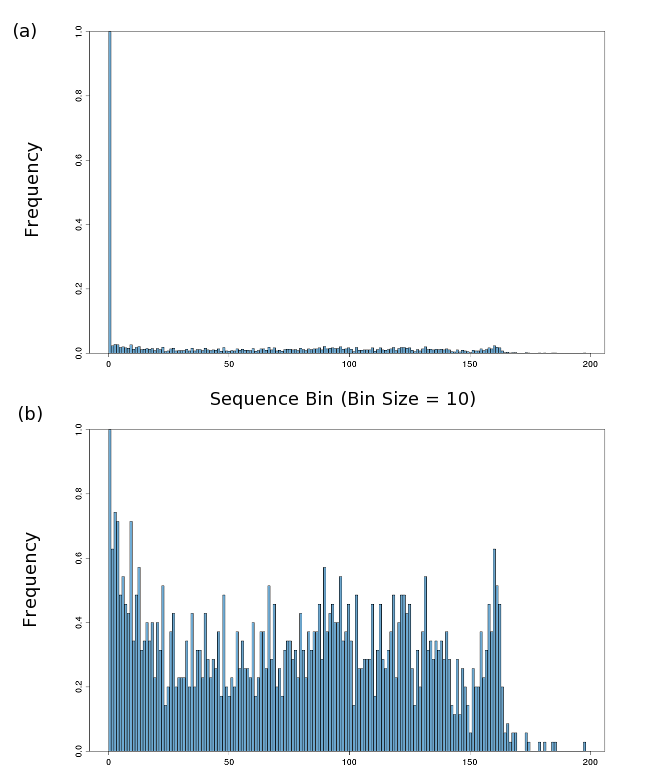
\includegraphics[angle=0, scale=0.8]{Chapter5/histocompare.png}
%\caption{Normalized  histograms showing  the  distribution of  overlap
%  values  in the  23S subunit  or \textit{Thermus  Thermophilus} rRNA,
%  PDB-ID:1jjk.  In  histogram (a)  all  values  are  included, but  in
%  histogram (b) only values greater than zero are included. Notice the
%  high preponderance  of zero  values, exactly 897  out of a  total of
%  2705.}
%\end{figure}
%For this case we obtain the dendrogram shown in Figure 1.2.
%\begin{figure}[htbp]
%\centering 
%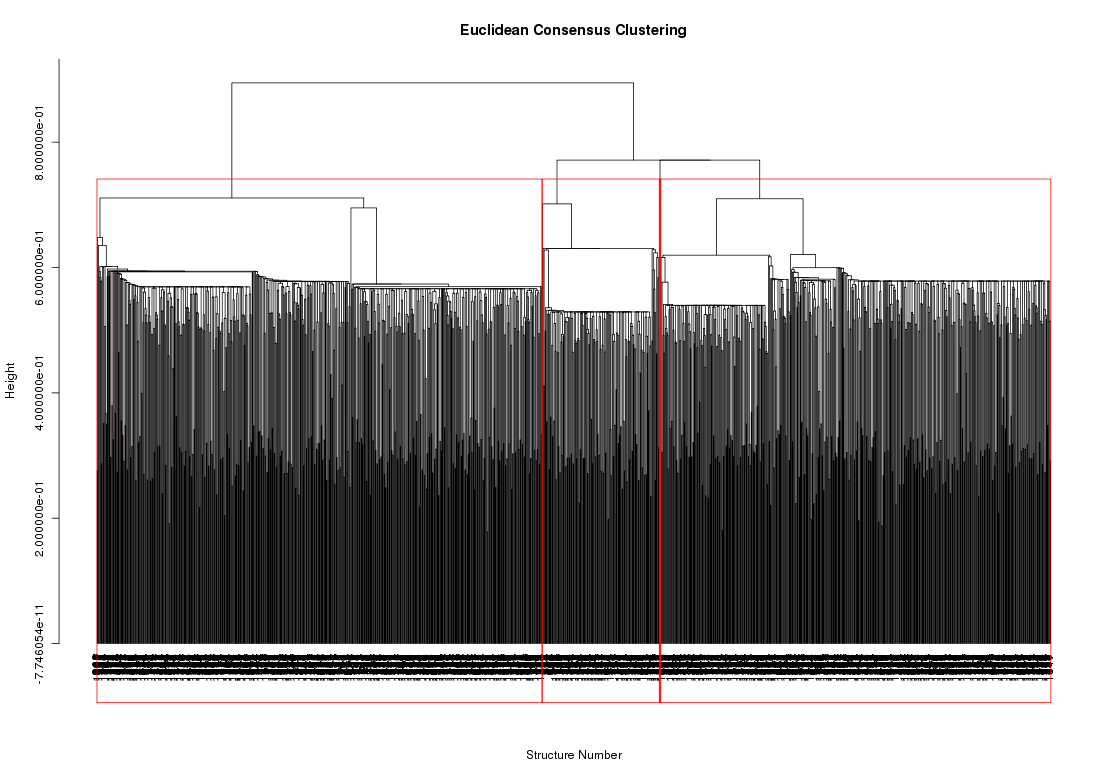
\includegraphics[angle=90, scale=0.6]{Chapter5/eucli_cons.png}
%\caption{Dendrogram for consensus clustering  of overlap scores in the
%  ribosome.  Zero values filtered out and remaining data normalized.}
%\end{figure}

%The next  step in this analysis  will be to find  the structures which
%correspond  to this  clusters  and superimpose  and  align them  using
%Kabsh's algorithm to be able to determine their RMSD's.

%Many people  start their  RNA Motif identification  and classification
%algorithms by splitting  RNA structures into what is  helical and what
%is not,  and then  finding interactions between  these two  groups. We
%believe that  we could do  a similar exercise  with 3DNA by  using the
%scalar  product   of  helical  axis  vectors  and   once  helical  and
%non-helical regions are  found we might be able to  use 3DNA Parser to
%look for characteristic interactions.

%\section{Triplets on RNA (comparison to Laing et al.)}

\section{Conclusions}
We  answer  the questions  at  the begining  of  this  chapter in  the
following way:

\begin{enumerate}
\item{\textbf{Q.}  Can   the  geometric  rigid-block   description  of
  base-pairing  and base-stacking  solve the  problem of  defining RNA
  structural motifs?}
\item{\textbf{A.}  The problem  of defining  RNA structural  motifs is
  clearly  more  complicated  than  what  can  be  understood  by  any
  structural  research  methodology  alone.  We have  shown  that  the
  rigid-body parameter view of RNA  can easily automate the process of
  motif  searches  in RNA  atomic  structures,  and  it helps  in  the
  description   of   motifs,    therefore   we   believe   that   this
  characterization should not be ignored by the community and included
  in ontological efforts such as the ROC one.}
\item{\textbf{Q.} Can we use quantities derived from the 3DNA software
  package to make and automatic search for a known motif, for example,
  the GNRA tetraloop motif, and perhaps find unknown motifs?}
\item{\textbf{A.} Yes. by defining seeds from known motifs we can find
new motifs in  the boundaries of known ones  via base-pairs steps. But
we  can also  do  other,  yet simpler,  not  as ``precise''  searches,
e.g. by clustering  the results of base overlaps.  Other searches have
not  been explored  but could  also be  useful, for  example exploring
helical  parameters like x-displacement,  y-displacement, inclination,
tip.} 
\end{enumerate}

\bibliography{biblio}

